% =============================================================================
% Double U-Net Architecture — Detailed U-shape style
% =============================================================================
% Same visual style as unet_architecture.tex but for Double U-Net
% Network 1: VGG-19 encoder + ASPP + SE-Conv decoder
% Network 2: SE encoder on gated input + ASPP + dual-skip decoder
% =============================================================================
\documentclass[border=8pt]{standalone}
\usepackage{tikz}
\usepackage{xcolor}
\usepackage{amsmath}
\usetikzlibrary{arrows.meta, positioning, calc, fit, backgrounds}

% ---------------------------------------------------------------------------
% Color palette
% ---------------------------------------------------------------------------
% Network 1
\definecolor{vggblue}{RGB}{100, 149, 237}       % VGG encoder
\definecolor{dec1green}{RGB}{120, 190, 140}      % Decoder 1
\definecolor{asppcolor}{RGB}{255, 165, 40}       % ASPP
% Network 2
\definecolor{enc2purple}{RGB}{175, 130, 210}     % SE encoder
\definecolor{dec2coral}{RGB}{230, 130, 120}      % Decoder 2
% Shared
\definecolor{poolred}{RGB}{220, 80, 60}
\definecolor{upgreen}{RGB}{60, 179, 113}
\definecolor{skipgray}{RGB}{170, 170, 170}
\definecolor{outputyellow}{RGB}{255, 193, 37}
\definecolor{bottleneck}{RGB}{70, 130, 180}
\definecolor{gatecolor}{RGB}{200, 60, 50}
\definecolor{bgnet1}{RGB}{235, 243, 255}
\definecolor{bgnet2}{RGB}{255, 238, 243}

% ---------------------------------------------------------------------------
% Styles
% ---------------------------------------------------------------------------
\tikzset{
    vggblock/.style={draw=vggblue!80!black, thick, fill=vggblue!25,
        minimum width=#1, minimum height=0.65cm, rounded corners=2pt,
        font=\scriptsize\sffamily, inner sep=2pt},
    d1block/.style={draw=dec1green!80!black, thick, fill=dec1green!25,
        minimum width=#1, minimum height=0.65cm, rounded corners=2pt,
        font=\scriptsize\sffamily, inner sep=2pt},
    asppblk/.style={draw=asppcolor!80!black, thick, fill=asppcolor!25,
        minimum width=#1, minimum height=0.65cm, rounded corners=2pt,
        font=\scriptsize\sffamily, inner sep=2pt},
    e2block/.style={draw=enc2purple!80!black, thick, fill=enc2purple!20,
        minimum width=#1, minimum height=0.65cm, rounded corners=2pt,
        font=\scriptsize\sffamily, inner sep=2pt},
    d2block/.style={draw=dec2coral!80!black, thick, fill=dec2coral!20,
        minimum width=#1, minimum height=0.65cm, rounded corners=2pt,
        font=\scriptsize\sffamily, inner sep=2pt},
    outblk/.style={draw=outputyellow!80!black, thick, fill=outputyellow!35,
        minimum width=#1, minimum height=0.65cm, rounded corners=2pt,
        font=\scriptsize\sffamily, inner sep=2pt},
    inblk/.style={draw=black!60, thick, fill=black!8,
        minimum width=#1, minimum height=0.65cm, rounded corners=2pt,
        font=\scriptsize\sffamily, inner sep=2pt},
    gateblk/.style={draw=gatecolor!70!black, thick, fill=gatecolor!12,
        minimum width=#1, minimum height=0.65cm, rounded corners=2pt,
        font=\scriptsize\sffamily, inner sep=2pt},
    % Arrows
    darr/.style={-{Stealth[length=3.5pt]}, thick, poolred},
    uarr/.style={-{Stealth[length=3.5pt]}, thick, upgreen},
    carr/.style={-{Stealth[length=3pt]}, thick, black!55},
    sk1/.style={-{Stealth[length=3.5pt]}, thick, skipgray, dashed},
    sk2/.style={-{Stealth[length=3.5pt]}, thick, enc2purple!50, densely dotted},
    garr/.style={-{Stealth[length=4pt]}, very thick, gatecolor},
    % Labels
    dl/.style={font=\tiny\sffamily, text=black!65},
    cl/.style={font=\tiny\sffamily\bfseries, text=black!85},
    ol/.style={font=\tiny\sffamily, text=black!55, fill=white,
        fill opacity=0.85, text opacity=1, inner sep=1pt, rounded corners=1pt},
    ttl/.style={font=\footnotesize\sffamily\bfseries, text=black!75},
}

% Block widths: 384->3.4cm, 192->2.6cm, 96->2.0cm, 48->1.5cm, 24->1.1cm

\begin{document}
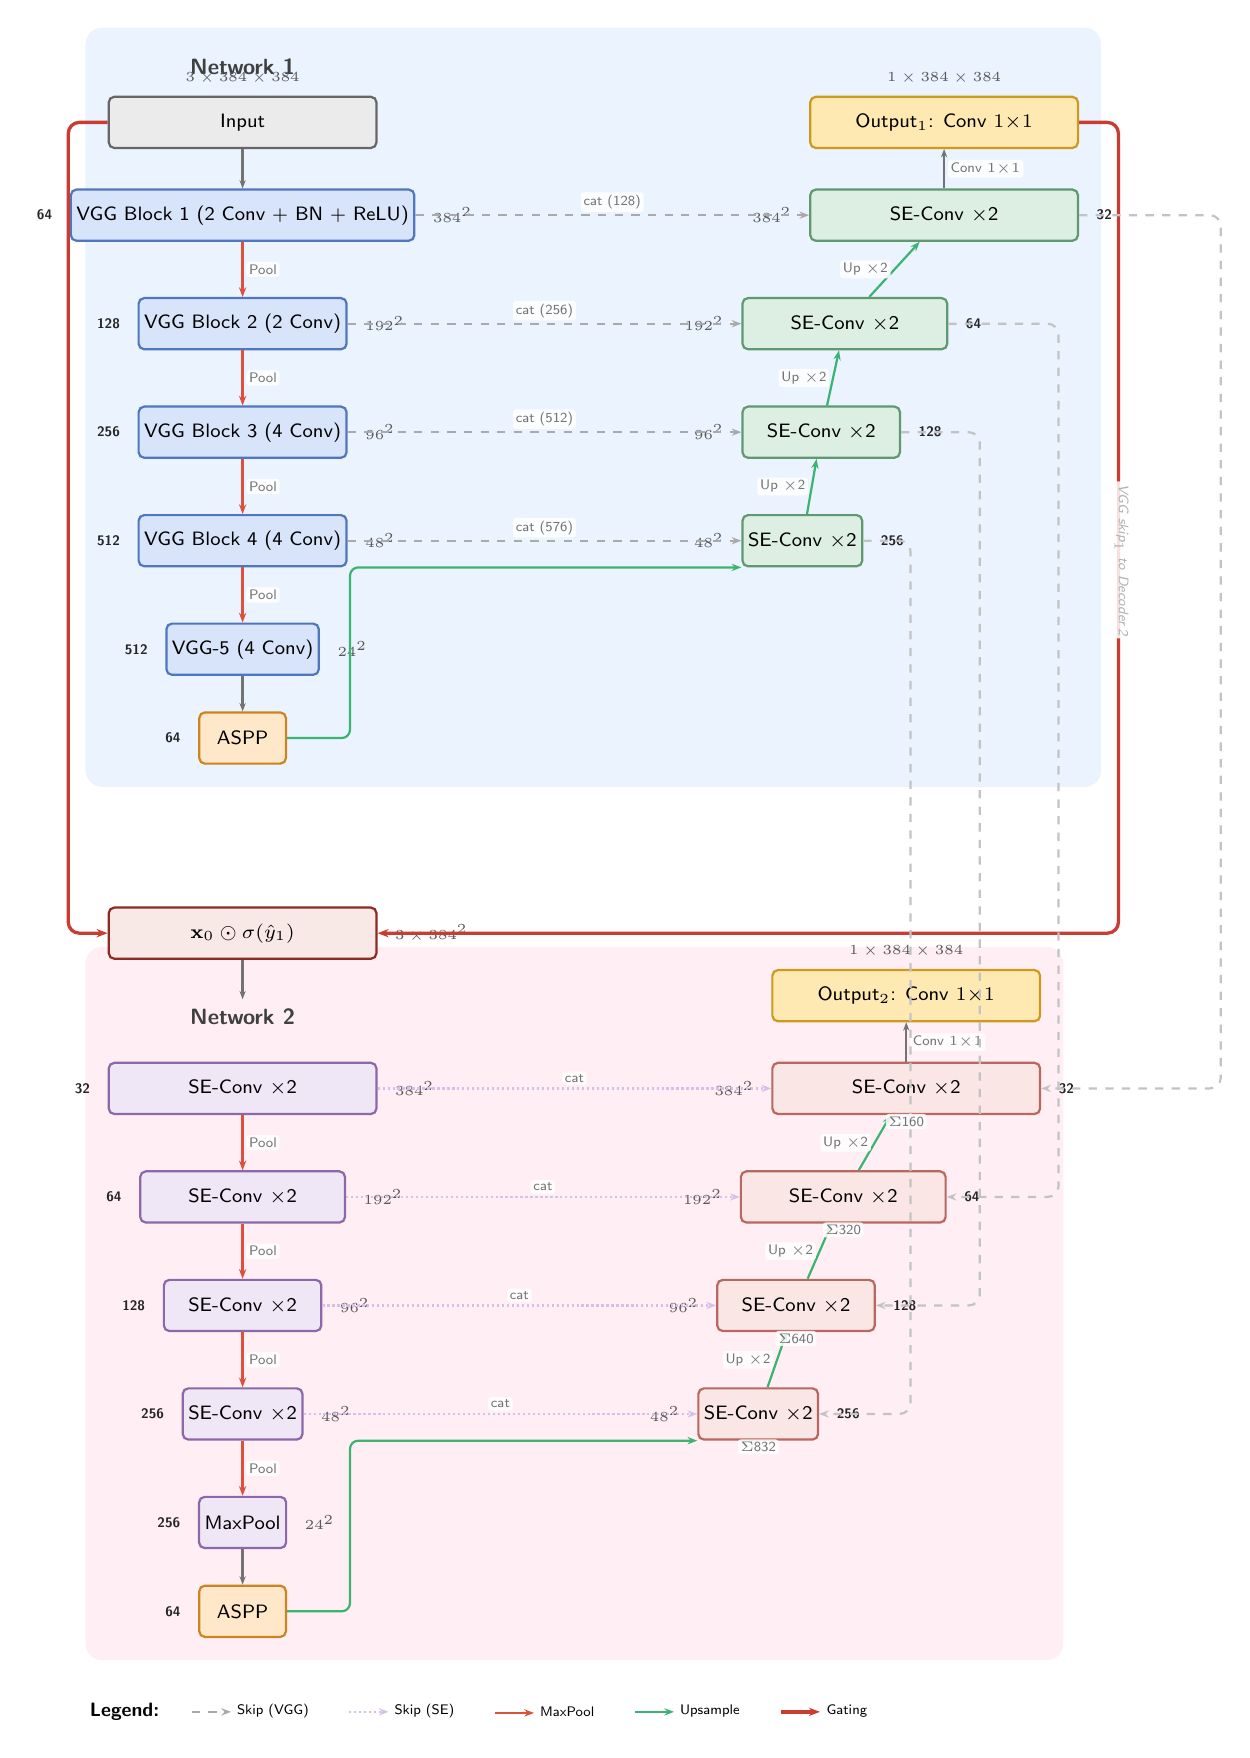
\begin{tikzpicture}[node distance=0.4cm]

% =====================================================================
%  NETWORK 1 — ENCODER (left, going down)
% =====================================================================
\node[ttl] (n1t) at (0, 0.7) {Network 1};

% Input
\node[inblk=3.4cm] (inp) at (0, 0) {Input};
\node[dl, above=0.03cm of inp] {$3 \times 384 \times 384$};

% VGG-1: 64 × 384²
\node[vggblock=3.4cm, below=0.5cm of inp] (v1) {VGG Block 1 (2 Conv + BN + ReLU)};
\node[cl, left=0.1cm of v1] {64};
\node[dl, right=0.1cm of v1] {$384^2$};

% VGG-2: 128 × 192²
\node[vggblock=2.6cm, below=0.7cm of v1] (v2) {VGG Block 2 (2 Conv)};
\node[cl, left=0.1cm of v2] {128};
\node[dl, right=0.1cm of v2] {$192^2$};

% VGG-3: 256 × 96²
\node[vggblock=2.0cm, below=0.7cm of v2] (v3) {VGG Block 3 (4 Conv)};
\node[cl, left=0.1cm of v3] {256};
\node[dl, right=0.1cm of v3] {$96^2$};

% VGG-4: 512 × 48²
\node[vggblock=1.5cm, below=0.7cm of v3] (v4) {VGG Block 4 (4 Conv)};
\node[cl, left=0.1cm of v4] {512};
\node[dl, right=0.1cm of v4] {$48^2$};

% VGG-5: 512 × 24²
\node[vggblock=1.1cm, below=0.7cm of v4] (v5) {VGG-5 (4 Conv)};
\node[cl, left=0.1cm of v5] {512};
\node[dl, right=0.1cm of v5] {$24^2$};

% ASPP 1: 64 × 24²
\node[asppblk=1.1cm, below=0.45cm of v5] (a1) {ASPP};
\node[cl, left=0.1cm of a1] {64};

% =====================================================================
%  NETWORK 1 — DECODER (right, going up)
% =====================================================================

% Dec1-1: 256 × 48² (same level as v4)
\node[d1block=1.5cm, right=5.0cm of v4] (d11) {SE-Conv $\times$2};
\node[cl, right=0.1cm of d11] {256};
\node[dl, left=0.1cm of d11] {$48^2$};

% Dec1-2: 128 × 96²
\node[d1block=2.0cm, right=5.0cm of v3] (d12) {SE-Conv $\times$2};
\node[cl, right=0.1cm of d12] {128};
\node[dl, left=0.1cm of d12] {$96^2$};

% Dec1-3: 64 × 192²
\node[d1block=2.6cm, right=5.0cm of v2] (d13) {SE-Conv $\times$2};
\node[cl, right=0.1cm of d13] {64};
\node[dl, left=0.1cm of d13] {$192^2$};

% Dec1-4: 32 × 384²
\node[d1block=3.4cm, right=5.0cm of v1] (d14) {SE-Conv $\times$2};
\node[cl, right=0.1cm of d14] {32};
\node[dl, left=0.1cm of d14] {$384^2$};

% Output 1
\node[outblk=3.4cm, above=0.5cm of d14] (o1) {Output$_1$: Conv $1{\times}1$};
\node[dl, above=0.03cm of o1] {$1 \times 384 \times 384$};

% --- Encoder arrows ---
\draw[carr] (inp) -- (v1);
\draw[darr] (v1) -- node[ol, right=1pt] {Pool} (v2);
\draw[darr] (v2) -- node[ol, right=1pt] {Pool} (v3);
\draw[darr] (v3) -- node[ol, right=1pt] {Pool} (v4);
\draw[darr] (v4) -- node[ol, right=1pt] {Pool} (v5);
\draw[carr] (v5) -- (a1);

% --- Bottleneck → Dec1-1 ---
\draw[uarr, rounded corners=3pt] (a1.east) -- ++(0.8,0) |- (d11.south west);

% --- Decoder arrows ---
\draw[uarr] (d11) -- node[ol, left=1pt] {Up $\times$2} (d12);
\draw[uarr] (d12) -- node[ol, left=1pt] {Up $\times$2} (d13);
\draw[uarr] (d13) -- node[ol, left=1pt] {Up $\times$2} (d14);
\draw[carr] (d14) -- node[ol, right=1pt] {Conv $1{\times}1$} (o1);

% --- Skip connections Net1 (horizontal) ---
\draw[sk1] (v4.east) -- (d11.west);
\node[ol] at ($(v4.east)!0.5!(d11.west)$) [above=1pt] {cat (576)};

\draw[sk1] (v3.east) -- (d12.west);
\node[ol] at ($(v3.east)!0.5!(d12.west)$) [above=1pt] {cat (512)};

\draw[sk1] (v2.east) -- (d13.west);
\node[ol] at ($(v2.east)!0.5!(d13.west)$) [above=1pt] {cat (256)};

\draw[sk1] (v1.east) -- (d14.west);
\node[ol] at ($(v1.east)!0.5!(d14.west)$) [above=1pt] {cat (128)};

% =====================================================================
%  GATING — between networks
% =====================================================================
\node[gateblk=3.4cm, below=1.8cm of a1] (gate)
  {$\mathbf{x}_0 \odot \sigma(\hat{y}_1)$};
\node[dl, right=0.1cm of gate] {$3 \times 384^2$};

% Input → Gate (left edge)
\draw[garr, rounded corners=4pt]
  (inp.west) -- ++(-0.5,0) |- (gate.west);

% Output1 → Gate (right edge)
\draw[garr, rounded corners=4pt]
  (o1.east) -- ++(0.5,0) |- (gate.east);

% =====================================================================
%  NETWORK 2 — ENCODER (left, going down)
% =====================================================================
\node[ttl, below=0.5cm of gate] (n2t) {Network 2};

% SE-1: 32 × 384²
\node[e2block=3.4cm, below=0.35cm of n2t] (s1) {SE-Conv $\times$2};
\node[cl, left=0.1cm of s1] {32};
\node[dl, right=0.1cm of s1] {$384^2$};

% SE-2: 64 × 192²
\node[e2block=2.6cm, below=0.7cm of s1] (s2) {SE-Conv $\times$2};
\node[cl, left=0.1cm of s2] {64};
\node[dl, right=0.1cm of s2] {$192^2$};

% SE-3: 128 × 96²
\node[e2block=2.0cm, below=0.7cm of s2] (s3) {SE-Conv $\times$2};
\node[cl, left=0.1cm of s3] {128};
\node[dl, right=0.1cm of s3] {$96^2$};

% SE-4: 256 × 48²
\node[e2block=1.5cm, below=0.7cm of s3] (s4) {SE-Conv $\times$2};
\node[cl, left=0.1cm of s4] {256};
\node[dl, right=0.1cm of s4] {$48^2$};

% Pool: 256 × 24²
\node[e2block=1.1cm, below=0.7cm of s4] (sp) {MaxPool};
\node[cl, left=0.1cm of sp] {256};
\node[dl, right=0.1cm of sp] {$24^2$};

% ASPP 2: 64 × 24²
\node[asppblk=1.1cm, below=0.45cm of sp] (a2) {ASPP};
\node[cl, left=0.1cm of a2] {64};

% =====================================================================
%  NETWORK 2 — DECODER (right, going up)
% =====================================================================

% Dec2-1: 256 × 48² (same level as s4)
\node[d2block=1.5cm, right=5.0cm of s4] (d21) {SE-Conv $\times$2};
\node[cl, right=0.1cm of d21] {256};
\node[dl, left=0.1cm of d21] {$48^2$};

% Dec2-2: 128 × 96²
\node[d2block=2.0cm, right=5.0cm of s3] (d22) {SE-Conv $\times$2};
\node[cl, right=0.1cm of d22] {128};
\node[dl, left=0.1cm of d22] {$96^2$};

% Dec2-3: 64 × 192²
\node[d2block=2.6cm, right=5.0cm of s2] (d23) {SE-Conv $\times$2};
\node[cl, right=0.1cm of d23] {64};
\node[dl, left=0.1cm of d23] {$192^2$};

% Dec2-4: 32 × 384²
\node[d2block=3.4cm, right=5.0cm of s1] (d24) {SE-Conv $\times$2};
\node[cl, right=0.1cm of d24] {32};
\node[dl, left=0.1cm of d24] {$384^2$};

% Output 2
\node[outblk=3.4cm, above=0.5cm of d24] (o2) {Output$_2$: Conv $1{\times}1$};
\node[dl, above=0.03cm of o2] {$1 \times 384 \times 384$};

% --- Gate → Encoder 2 ---
\draw[carr] (gate) -- (n2t);

% --- Encoder 2 arrows ---
\draw[darr] (s1) -- node[ol, right=1pt] {Pool} (s2);
\draw[darr] (s2) -- node[ol, right=1pt] {Pool} (s3);
\draw[darr] (s3) -- node[ol, right=1pt] {Pool} (s4);
\draw[darr] (s4) -- node[ol, right=1pt] {Pool} (sp);
\draw[carr] (sp) -- (a2);

% --- Bottleneck → Dec2-1 ---
\draw[uarr, rounded corners=3pt] (a2.east) -- ++(0.8,0) |- (d21.south west);

% --- Decoder 2 arrows ---
\draw[uarr] (d21) -- node[ol, left=1pt] {Up $\times$2} (d22);
\draw[uarr] (d22) -- node[ol, left=1pt] {Up $\times$2} (d23);
\draw[uarr] (d23) -- node[ol, left=1pt] {Up $\times$2} (d24);
\draw[carr] (d24) -- node[ol, right=1pt] {Conv $1{\times}1$} (o2);

% --- Skip connections Encoder2 → Decoder2 (purple dotted) ---
\draw[sk2] (s4.east) -- (d21.west);
\node[ol] at ($(s4.east)!0.5!(d21.west)$) [above=1pt] {cat};

\draw[sk2] (s3.east) -- (d22.west);
\node[ol] at ($(s3.east)!0.5!(d22.west)$) [above=1pt] {cat};

\draw[sk2] (s2.east) -- (d23.west);
\node[ol] at ($(s2.east)!0.5!(d23.west)$) [above=1pt] {cat};

\draw[sk2] (s1.east) -- (d24.west);
\node[ol] at ($(s1.east)!0.5!(d24.west)$) [above=1pt] {cat};

% --- Cross-network skip: VGG → Decoder2 (routed on far right) ---
% These carry VGG features to Decoder 2 as well (dual skip)
% Route along right edge to avoid crossing horizontal skip connections

\draw[sk1, skipgray!70, rounded corners=4pt]
  (d11.east) -- ++(0.6,0) |- (d21.east);
\draw[sk1, skipgray!70, rounded corners=4pt]
  (d12.east) -- ++(1.0,0) |- (d22.east);
\draw[sk1, skipgray!70, rounded corners=4pt]
  (d13.east) -- ++(1.4,0) |- (d23.east);
\draw[sk1, skipgray!70, rounded corners=4pt]
  (d14.east) -- ++(1.8,0) |- (d24.east);

% Label for cross-network skips
\node[ol, text=skipgray!90, font=\tiny\sffamily\itshape, rotate=-90]
  at ($(d13.east) + (2.2, -3.0)$) {VGG skip$_1$ to Decoder\,2};

% --- Total concat channels for Decoder 2 ---
\node[ol] at ($(d21.south) + (0, -0.08)$) {$\Sigma$832};
\node[ol] at ($(d22.south) + (0, -0.08)$) {$\Sigma$640};
\node[ol] at ($(d23.south) + (0, -0.08)$) {$\Sigma$320};
\node[ol] at ($(d24.south) + (0, -0.08)$) {$\Sigma$160};

% =====================================================================
%  Background boxes
% =====================================================================
\begin{scope}[on background layer]
  \node[fill=bgnet1, rounded corners=6pt,
        fit=(n1t)(inp)(v5)(a1)(o1)(d14),
        inner sep=8pt] {};
  \node[fill=bgnet2, rounded corners=6pt,
        fit=(n2t)(s1)(sp)(a2)(o2)(d24),
        inner sep=8pt] {};
\end{scope}

% =====================================================================
%  LEGEND
% =====================================================================
\node[anchor=north west, font=\scriptsize\sffamily\bfseries]
  at ($(a2.south west) + (-1.5, -0.7)$) (lt) {Legend:};

\node[right=0.15cm of lt, anchor=west, font=\tiny\sffamily] (l1) {%
  \tikz[baseline=-0.5ex]{\draw[sk1] (0,0) -- (0.5,0);} Skip (VGG)};
\node[right=0.25cm of l1, anchor=west, font=\tiny\sffamily] (l2) {%
  \tikz[baseline=-0.5ex]{\draw[sk2] (0,0) -- (0.5,0);} Skip (SE)};
\node[right=0.25cm of l2, anchor=west, font=\tiny\sffamily] (l3) {%
  \tikz[baseline=-0.5ex]{\draw[darr] (0,0) -- (0.5,0);} MaxPool};
\node[right=0.25cm of l3, anchor=west, font=\tiny\sffamily] (l4) {%
  \tikz[baseline=-0.5ex]{\draw[uarr] (0,0) -- (0.5,0);} Upsample};
\node[right=0.25cm of l4, anchor=west, font=\tiny\sffamily] (l5) {%
  \tikz[baseline=-0.5ex]{\draw[garr] (0,0) -- (0.5,0);} Gating};

\end{tikzpicture}
\end{document}
